\documentclass[10pt]{article}
\usepackage[a4paper, margin=1cm]{geometry}
\usepackage{
  fontspec,
  multicol,
  graphicx,
  enumitem,  % for \begin{itemize}[noitemsep, nolistsep] etc.
  hanging,
  tabularx,
  dblfnote
}

\setmainfont{Avenir}
\setlength{\parskip}{0.33em}

\pagestyle{empty}
\raggedright
\DFNalwaysdouble


\begin{document}

{\huge \textbf{Ruan van Mazijk}}~~{\Large \textit{Curriculum vitae}}
              \hfill \href{mailto:ruanvmazijk@gmail.com}{ruanvmazijk@gmail.com},
                                                               (+27) 72 516 7570

\vskip10pt \hrule \vskip2pt \hrule


\begin{multicols}{2} % =========================================================

\begin{hangparas}{2em}{1}

\textbf{MSc candidate} in Biological Sciences {\small
  (UCT\footnote{University of Cape Town})}                                \\
                                                    %\hfill {\small 2018--}
\hspace{2em} \textit{Genome-size effects on plant
  hydraulic ecophysiology, habitat \& phenology in
  Cape schoenoid sedges}                                                  \\
\hspace{2em} Principal supervisor: Prof A.M. Muasya.
  Co-supervisors: A/Prof G.A. Verboom \&
  A/Prof A.G. West

\textbf{BSc Hons} in Biological Sciences {\small
  (UCT) \textit{With distinction}}.                  \hfill {\small 2017} \\
\hspace{2em} \textit{Relating vascular plant species
  richness \& environmental heterogeneity spatially
  in the GCFR \& SWAFR}                                                   \\
\hspace{2em} Supervisors: Prof M.D. Cramer \&
  A/Prof G.A. Verboom

\textbf{BSc} in Ecology \& Evolution, Applied
  Biology {\small (UCT) \textit{With distinction in
  both majors \& the degree}}                        \hfill {\small 2016}

\end{hangparas}


\columnbreak

\textbf{Skills   }     \hfill      Strong speaker, design, data visualisation

\textbf{Languages}     \hfill   English, Afrikaans, \texttt{R}, \texttt{bash}

\textbf{Tools    }     \hfill \texttt{R} Markdown, {\fontfamily{lmr} \selectfont
                              \LaTeX}, \texttt{git}, GitHub, MS Office

\textbf{Methods  }     \hfill       Statistical modelling, data manipulation, \\
                       \hfill     GIS (in \texttt{R}), functional programming

\end{multicols} % ==============================================================

\hrule

\subsection*{Publications} % ---------------------------------------------------

\begin{hangparas}{2em}{1}

\textbf{Van Mazijk}, Cramer, \& Verboom. 2021.
Environmental heterogeneity explains contrasting plant species richness between
the South African Cape and southwestern Australia. \textit{J.~Biogeogr.~}
48:1875--1888. DOI: \href{https://doi.org/10.1111/jbi.14118}{10.1111/jbi.14118}.

Elliott, \textbf{van Mazijk}, Barrett, Bruhl, Joly,
Muthaphuli, Wilson, \& Muasya. 2021. Global dispersal and
diversification of the genus \textit{Schoenus} (Cyperaceae) from the Western
Australian biodiversity hotspot. \textit{J.~Syst.~\& Evol.~} 59(4):791--808. DOI:
\href{https://doi.org/10.1111/jse.1274}{10.1111/jse.12742}

Elliott, Laidler, Muasya, Muthaphuli \& \textbf{van Mazijk}. 2019. Solving the
sedge mystery. \textit{Veld \& Flora} 105(3):20--25. (Popular article)

Cramer, Wootton, \textbf{van Mazijk} \& Verboom. 2019.
New regionally-modelled soil layers improve prediction of vegetation type
relative to that based on global soil models. \textit{Divers.~Distrib.~}
25(11):1736--1750. DOI:
\href{https://doi.org/10.1111/ddi.12973}{10.1111/ddi.12973}.

\textbf{Van Mazijk}, Smyth, Weideman \& West. 2018.
Isotopic tracing of stormwater in the urban Liesbeek River. \textit{Water SA}
44(4):674--679. DOI:
\href{https://doi.org/10.4314/wsa.v44i4.16}{10.4314/wsa.v44i4.16}.

\end{hangparas}


\hrulefill

\begin{multicols}{2} % =========================================================

\subsection*{Funding \& awards} % ----------------------------------------------

NRF Innovation Masters Scholarship                       \hfill {\small 2019} \\
SAAB MSc Student Bursary {\small (inaugural recipient)}
                                                   \hfill {\small 2018, 2019} \\
UCT Once-Off Award                                 \hfill {\small       2018} \\
UCT Dorothy Cameron Scholarship                    \hfill {\small       2018} \\
UCT Masters Research Scholarship                   \hfill {\small       2018} \\
NRF Innovation Honours Scholarship                 \hfill {\small       2017} \\
SAAB Honours Scholarship                           \hfill {\small       2017} \\
UCT Science Faculty Scholarship                    \hfill {\small 2015, 2016}

\subsection*{Conferences, talks \& press} % ------------------------------------

SAAB Postgraduate Virtual Symposium                      \hfill {\small 2022} \\
MEDECOS XVII {\small (NRF sponsored virtual attendance)} \hfill {\small 2022} \\
IBS\footnote{International Biogeography Society}
  Early Career Biogeographers Conference                 \hfill {\small 2021} \\
iDiv\footnote{
    German Centre for Integrative Biodiversity Research, Halle-Jena-Leipzig}
  Joint Recruitment Symposium                            \hfill {\small 2020} \\
SAAB\footnote{
    South African Association of Botanists}-AMA\footnote{
      African Mycological Association}-SASSB\footnote{
        Southern African Society for Systematic Biology}
  IVXV Joint Congress                                    \hfill {\small 2019} \\
  \hspace{2em} {\small Best Systematics MSc Presentation (tied)}              \\
  \hspace{2em} {\small (UCT Travel Grant for attendance)}                     \\
The John Maytham Show, CapeTalk     {\small (Interview)} \hfill {\small 2018} \\
  \hspace{2em} {\small \href{https://www.capetalk.co.za/articles/328900/harvesting-stormwater-from-liesbeek-river-may-aid-ct-water-supply-students-find}
                            {\textit{Harvesting Storm Water}}}                \\
Pint of Science Cape Town                                \hfill {\small 2018}

\columnbreak

\subsection*{Workshop instruction % --------------------------------------------
                                 \hfill {\small \textmd{\textit{Postgraduate}}}}

Data wrangling \& manipulation in \texttt{R}
  {\small (Organiser,}                             \hfill {\small       2019} \\
  \hspace{2em} {\small lead, for Dept.~Biological
    Sciences, UCT)}                                                           \\
Teaching Biodiversity for High School              \hfill {\small       2019} \\
  \hspace{2em} Life Science Teachers {\small
    (Speaker, for SDU\footnote{Schools Development
    Unit, UCT})}                                                              \\
Scientific study design \& data analysis in \texttt{R}                        \\
  \hspace{2em} {\small(Tutor, for SEEC\footnote{
    Centre for Statistics in Ecology, the
    Environment \& Conservation, UCT}-ACCESS\footnote{
      Applied Centre for Climate \& Earth Systems,
      NRF})}                                       \hfill {\small 2018, 2019}

\subsection*{Teaching assistance % ---------------------------------------------
                                \hfill {\small \textmd{\textit{Undergraduate}}}}

Angiosperm diversity                         \hfill {\small 2018, 2019, 2022} \\
Principles of ecology \& evolution           \hfill {\small       2019, 2020} \\
Scientific study design \& data analysis in \texttt{R}
                                             \hfill {\small       2017--2020} \\
                              % NOTE: finished tutoring for STA2007* in Aug 2020
Introductory statistics in \texttt{R}        \hfill {\small       2016--2018}

\subsection*{References % ------------------------------------------------------
           \hfill {\small \textmd{\textit{All Dept.~Biological Sciences, UCT}}}}

Prof G.~Anthony Verboom
      \hfill     \href{mailto:tony.verboom@uct.ac.za}{tony.verboom@uct.ac.za} \\
Prof Michael D.~Cramer
      \hfill \href{mailto:michael.cramer@uct.ac.za}{michael.cramer@uct.ac.za} \\
Prof A.~Muthama Muasya
      \hfill \href{mailto:muthama.muasya@uct.ac.za}{muthama.muasya@uct.ac.za} \\
%Prof Adam G.~West
%      \hfill           \href{mailto:adam.west@uct.ac.za}{adam.west@uct.ac.za} \\

\begin{multicols}{2}
  \subsection*{\normalsize Professional affiliations} % ------------------------
  SAAB                       \hfill {\small 2017--\hspace*{2.5em}} \\
  SASSB                      \hfill {\small 2018--\hspace*{2.5em}} \\
  \hspace{1em} (Student rep. \hfill {\small 2019--2021})
  \vfill
  \columnbreak
  \begin{center}
    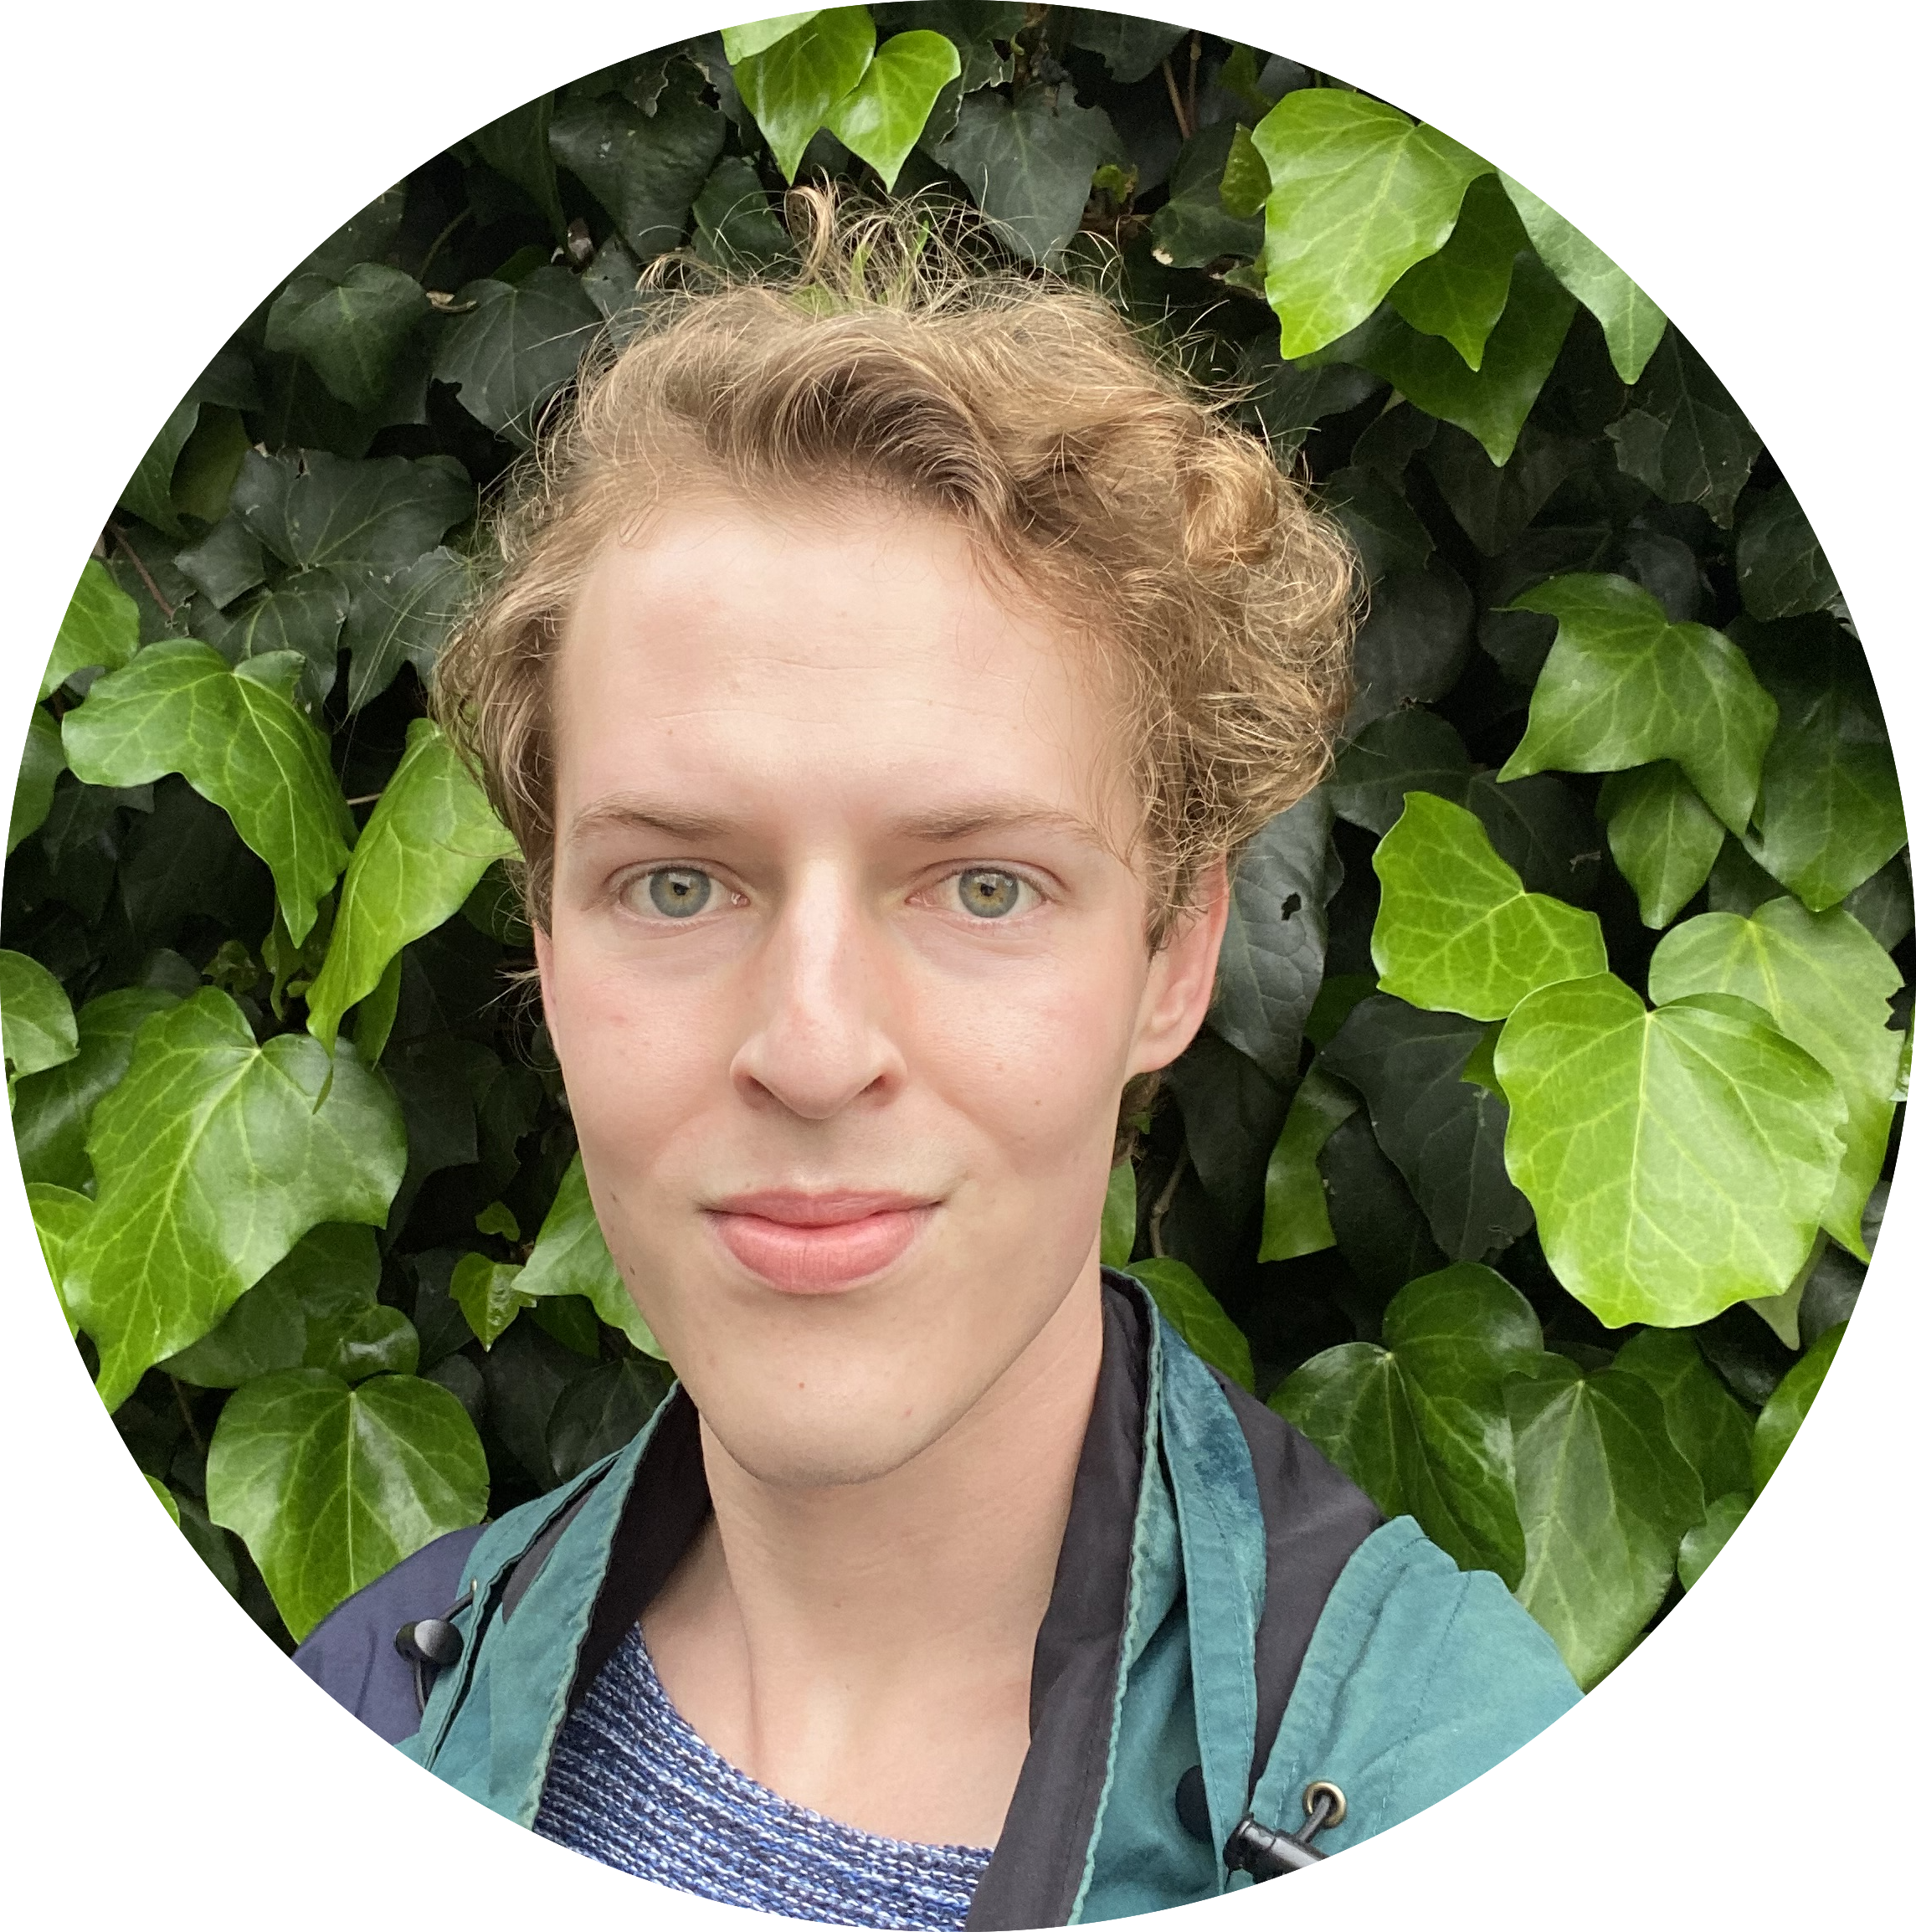
\includegraphics[width=10em]{IMG_4958_crop.png}
  \end{center}
\end{multicols}

\end{multicols} % ==============================================================

\subsection*{Research assistance} % --------------------------------------------

\textit{Schoenus} (Cyperaceae)
  field assistance, collections \& hydroponics
  for Dr T.L.~Elliott \& Prof A.M.~Muasya
  {\small (UCT)}                                         \hfill {\small 2018} \\
\textit{Mimetes} \& \textit{Leucospermum} (Proteaceae)
  population monitoring
  for Dr J.A.~Slingsby
  {\small (UCT, SAEON)}                                  \hfill {\small 2017} \\
Legume symbiotic rhizobia
  collections \& culturing
  for Dr M.~Dludlu
  {\small (University of Swaziland)}                     \hfill {\small 2015}

\end{document}
